\documentclass{article}
\usepackage[utf8]{inputenc} % Permite el uso de caracteres del Español
\usepackage[T1]{fontenc}
\usepackage{hyperref}
\usepackage{graphicx}
\usepackage{wrapfig}
\usepackage{subcaption}

% set font encoding for PDFLaTeX or XeLaTeX
\usepackage{ifxetex}
\ifxetex
  \usepackage{fontspec}
\else
  \usepackage[T1]{fontenc}
  \usepackage[utf8]{inputenc}
  \usepackage{lmodern}
\fi

% used in maketitle
\title{Evalución 1: Análisis de las mareas y salinidad en el Manglar El Sargento.}
\author{Melissa Matrecitos Avila}
\date{8 de Marzo de 2018}

% Enable SageTeX to run SageMath code right inside this LaTeX file.
% documentation: http://mirrors.ctan.org/macros/latex/contrib/sagetex/sagetexpackage.pdf
% \usepackage{sagetex}

\begin{document}
\maketitle
\section{Preparación de datos}
Para comenzar se descargaron dos archivos que contenían los datos a estudiar, los documentos fueron:
\begin{center}
    \includegraphics[width=.3\textwidth]{ArchivosDescargados.png}
\end{center}
Los cuales tienen la siguiente estructura, el primero corresponde al archivo con nombre sargento\_201117.csv y el segundo a sargento\-salinidad\-201117.csv:
\begin{center}
    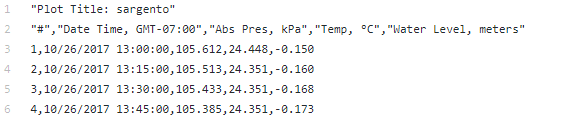
\includegraphics[width=.8\textwidth]{Datos_sargento.PNG}
    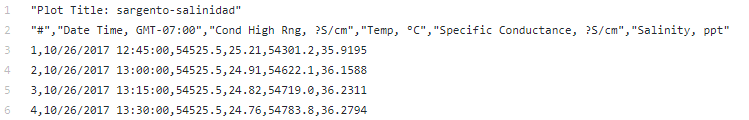
\includegraphics[width=1\textwidth]{Datos_Salinidad.PNG}
\end{center}
Para poder trabajar con ellos en pandas, se les cambió el nombre, eliminando los guiones o cambiándolos por guión bajo.
Procediendo en el entorno de jupyter notebook, lo primero que se hizo fue importar las bibliotecas que se utilizarían más adelate:
\begin{center}
    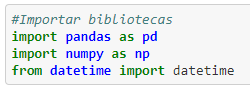
\includegraphics[width=.4\textwidth]{Bibliotecas.PNG}
\end{center}
Posteriormente se leyeron los dos archivos que contenían los datos, saltando los dos primeros renglones ya que no contenían datos, además se la asignaron los nombres a las columnas de cada archivo:
\begin{center}
    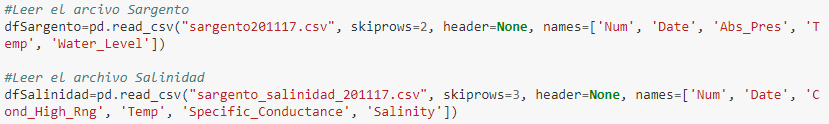
\includegraphics[width=1\textwidth]{Lectura.PNG}
\end{center}
Continuando con la preparación de los datos, se imprimió en la pantalla las dos cabezas y finales de ambas tablas, con el fin de verificar que ambas tuvieran el mismo número de datos, cómo no fue así, se eliminaron los datos extras en el archivo de nombre "sargento", logrando que los dos archivos constaran de la misma cantidad. La siguiente imagen muestra el final de la tabla Sargento (los últimos 5 datos), donde se muestra la cantidad de datos que ésta tiene:
\begin{center}
    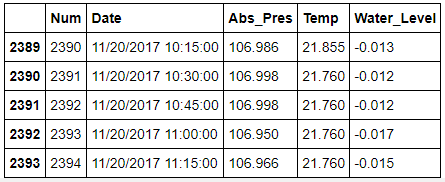
\includegraphics[width=.5\textwidth]{Final_tabla.PNG}
\end{center}
Por último, se creo para cada archivo, dos columnas nuevas, de tipo "date", que contenían la fecha y el mes en el que se tomarón los datos, esto con el fin de poder trabajar con los datos en las bibliotecas mencionadas anteriormente:
\begin{center}
    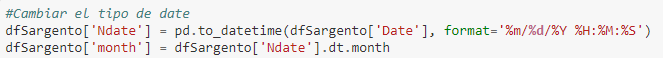
\includegraphics[width=.7\textwidth]{TipoDate.PNG}
\end{center}
La imagen anterior muestra la instrucción para realizar las acciones mencionadas, solo se muestra para el archivo "sargento", ya que fue lo mismo que se realizó para el archivo "salinidad".
El formato final de los datos , pra el archivo sargento y salinidad respectivamente, fue:
\begin{center}
    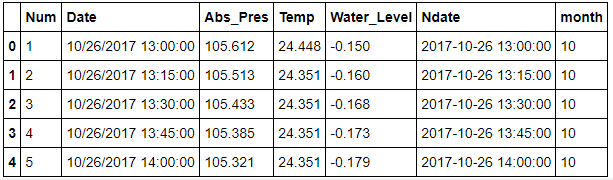
\includegraphics[width=.7\textwidth]{DatosListosS.PNG}
    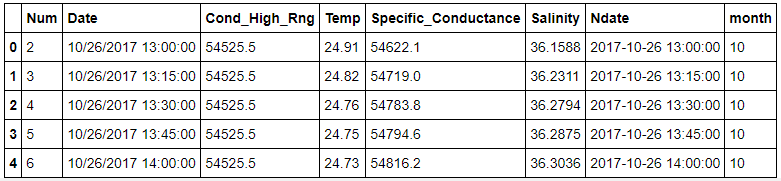
\includegraphics[width=.8\textwidth]{DatosListosSS.PNG}
\end{center}
\section{Análisis y Resultados de los Datos}
Para conocer el comportamiento de las variables a estudiar, se realizaron distintos diagramas que nos proporcionan información muy valiosa. Para los diagramas de caja y Correlación de Pearson se utilizó la biblioteca de Seaborn, mientras que para las demás se usó la biblioteca Matplotlib. la cual nos da más libertad para manejar los datos, siendo las gráficas supuestas las más complejas. A continuación se muestra el código que se utilizó para crear cada uno de los diagramas y su diagrama correspondiente, siendo el primer código que aparece el creador del primer diagrama:
\begin{itemize}
\item \textbf{Diagrama de caja}:


Para el estudio de cada variable se crearon dos cajas, la cuales corresponden al mes de octubre y noviembre. Las variables a estudiar fueron nivel del mar, salinidad y temperatura, todas contra tiempo.
\begin{center}
    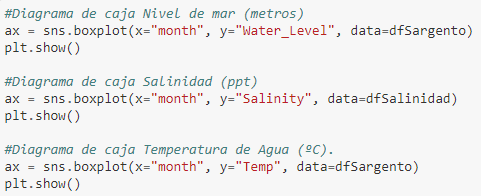
\includegraphics[width=.6\textwidth]{Diagramadecaja.PNG}
    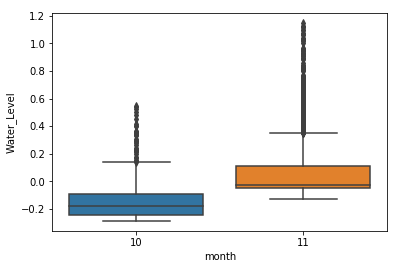
\includegraphics[width=.5\textwidth]{DC1.PNG}
    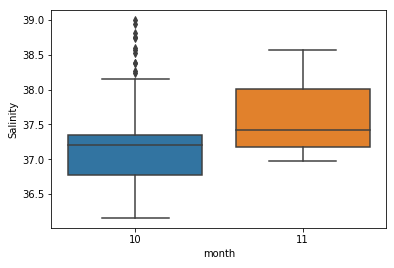
\includegraphics[width=.5\textwidth]{DC2.PNG}
    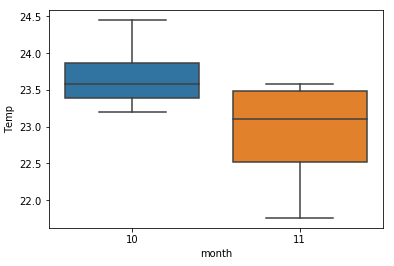
\includegraphics[width=.5\textwidth]{DC3.PNG}
\end{center}
\item \textbf{Describe}:


Este comando se utilizo como un apoyo para loa diagramas de caja, dando a conocer valores importantes más exactos:
\begin{center}
    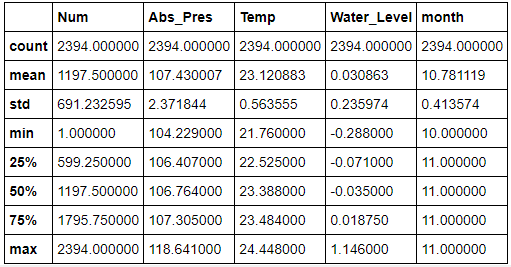
\includegraphics[width=.6\textwidth]{DescribeS.PNG}
    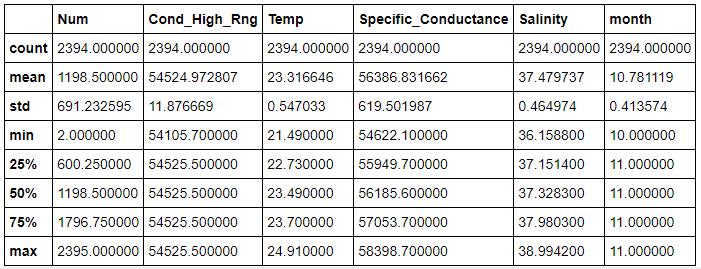
\includegraphics[width=.8\textwidth]{DescribeSS.PNG}
\end{center}

\item \textbf{Correlación Pearson}:

Para llevar a cabo la primera gráfica fue necesario guardar los datos de interés un nuevo Data Frame donde se combinaran los datos de Sargento y Salinidad. En la primera gráfica se muestra la relación de entre nivel de mar y salinidad, en la segunda nivel de mar y temperatura del agua y en la última salinidad y temperatura del agua:
\begin{center}
    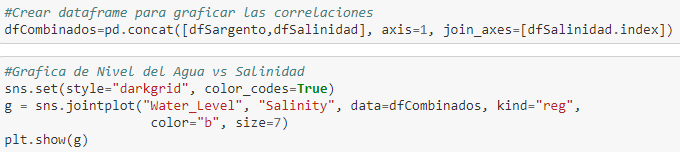
\includegraphics[width=.8\textwidth]{CPearson1.PNG}
    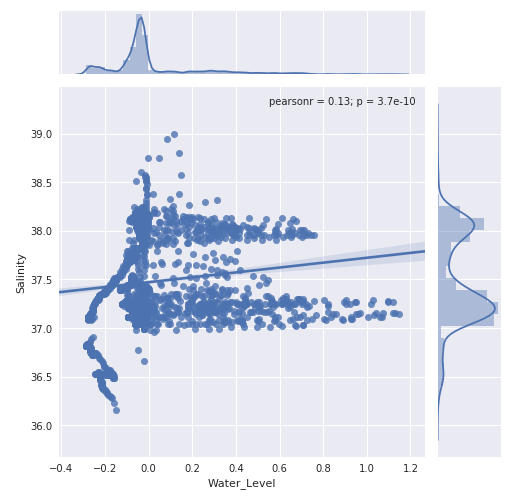
\includegraphics[width=.6\textwidth]{Pearson1.PNG}
    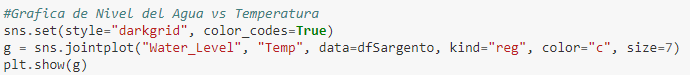
\includegraphics[width=.8\textwidth]{CPearson2.PNG}
    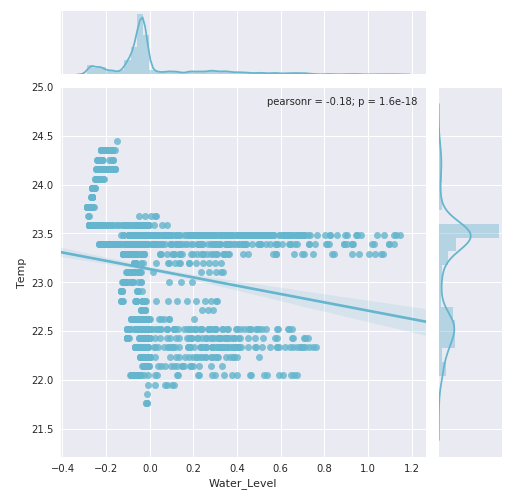
\includegraphics[width=.6\textwidth]{Pearson2.PNG}
    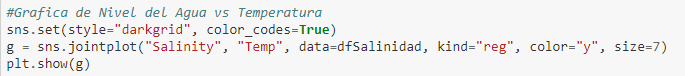
\includegraphics[width=.8\textwidth]{CPearson3.PNG}
    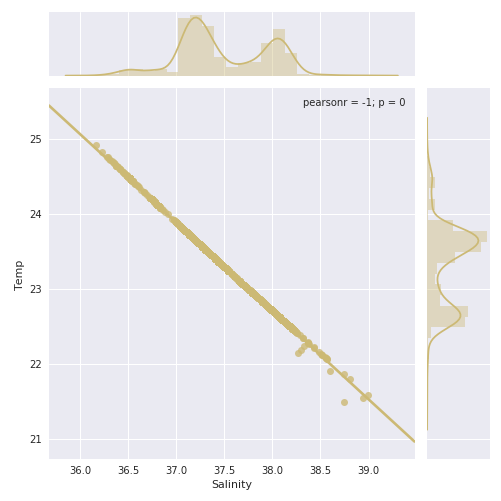
\includegraphics[width=.6\textwidth]{Pearson3.PNG}
\end{center}
\item \textbf{Gráficas Independietes}:


En esta actividad se realizaron 3 gráficas independientes de las variables nivel del mar, salinidad y temperatura del agua (respectivamente), para ver como cambiaban en función del tiempo.
\begin{center}
    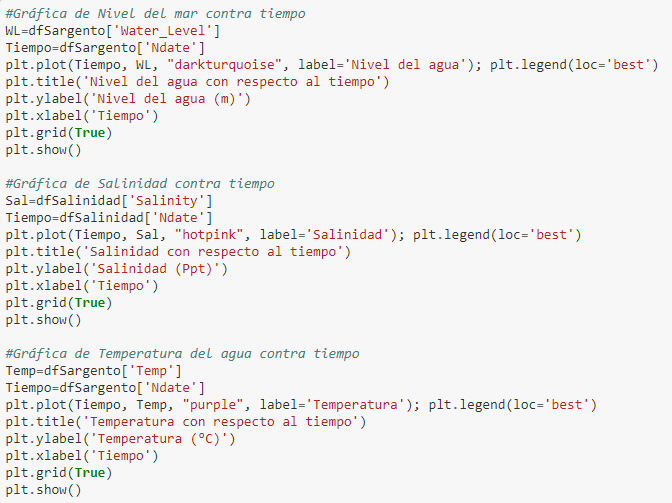
\includegraphics[width=.8\textwidth]{Independientes.PNG}
    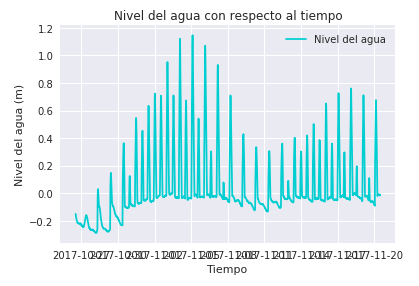
\includegraphics[width=.5\textwidth]{I1.PNG}
    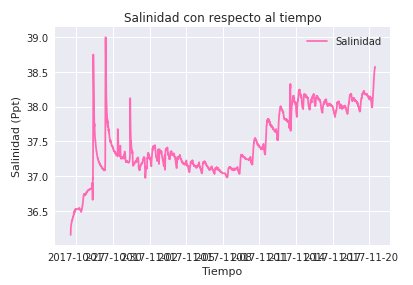
\includegraphics[width=.5\textwidth]{I2.PNG}
    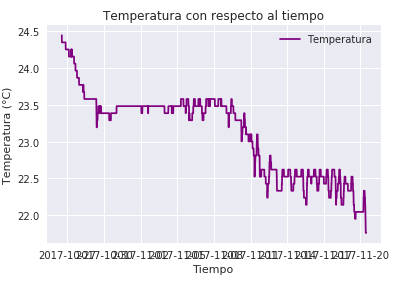
\includegraphics[width=.5\textwidth]{I3.PNG}
\end{center}
\item \textbf{Gráficas supuestas}:


Las gráficas realizadas en esta sección muestran el comportamiento de dos variables con respecto a una misma, las variables a estudiar por gráfica fueron: nivel de mar y salinidad y en la otra nivel de mar y temperatura. Este tipo de gráficas no sin las convencionales de Matplotlib, por lo que tienen un estructura distinta, tal como se muestra en el código:
\begin{center}
    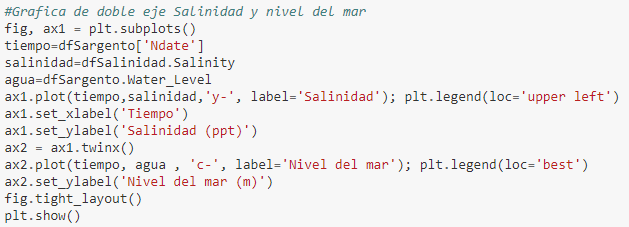
\includegraphics[width=.8\textwidth]{Supuestas1.PNG}
    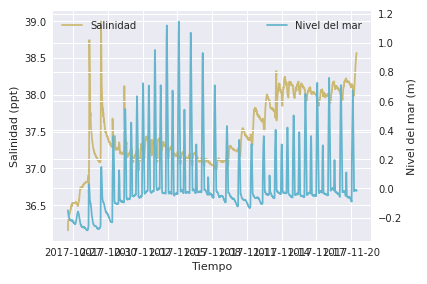
\includegraphics[width=.5\textwidth]{S1.PNG}
    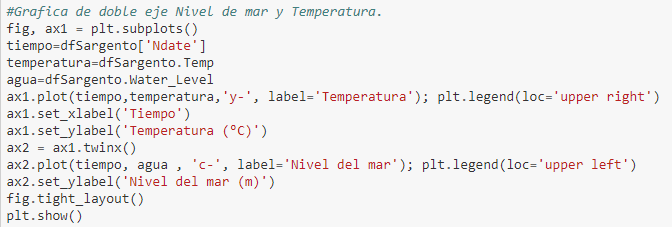
\includegraphics[width=.8\textwidth]{Supuestas2.PNG}
    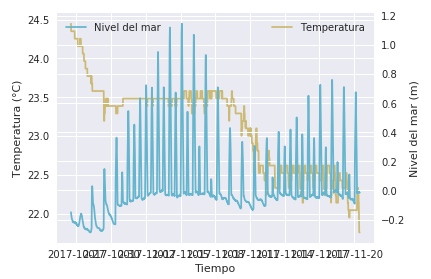
\includegraphics[width=.5\textwidth]{S2.PNG}
\end{center}
\item \textbf{Gráficas Independientes con xlim}:


Para poder observar mejor el comportamiento de las variables estudiadas en la parte anterior, se utilizo el comando xlim, para tener un rango de datos más pequeño que estudiar, tomando un rango de 5 días, que van del 26 de octubre al 31 del mismo mes:
\begin{center}
    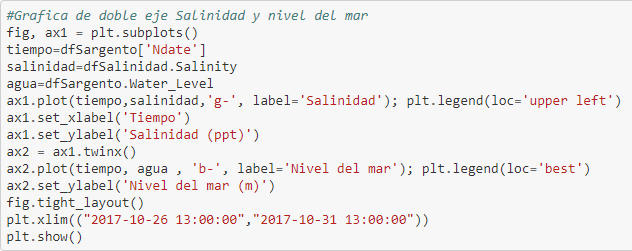
\includegraphics[width=.8\textwidth]{Independientesxlim1.PNG}
    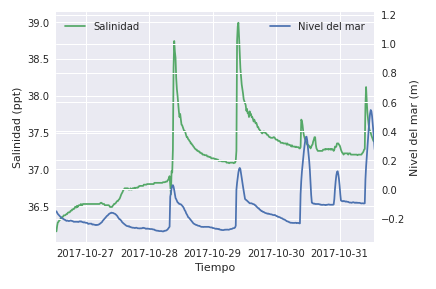
\includegraphics[width=.5\textwidth]{Ix1.PNG}
    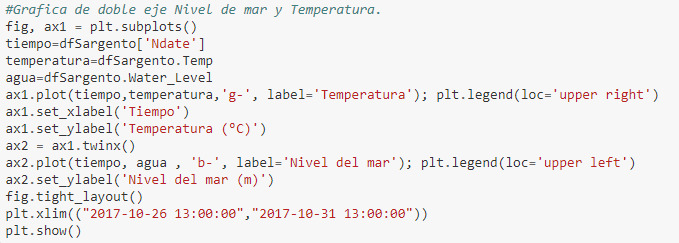
\includegraphics[width=.8\textwidth]{Independientesxlim2.PNG}
    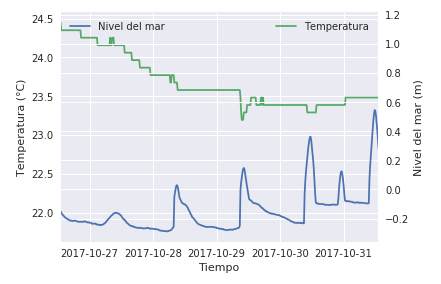
\includegraphics[width=.5\textwidth]{Ix2.PNG}
\end{center}
En la primera gráfica se puede observar claramente la relación , ya que los picos de una variable corresponden a los picos de la otra. Mientras que en la segunda gráfica se observa como mientras el nivel del mar aumenta, la temperatura va disminuyendo.
\end{itemize}

\section{Conclusión}
Con esta evaluación me doy cuenta de lo mucho que he aprendido en lo que va del semestre, pero sobre todo, lo mucho que me falta, ya que las bibliotecas pueden tener muchas funciones que facilitan el análisis de los datos.

Me gustaron mucho las actividades realizadas y espero haberlas completado correctamente.
\end{document}
